% -*- coding: utf-8 -*-

\section{Introduction}
\label{introduction}

The area of protein folding (and from this the creation of newer and better drugs) with the aid of computers, has since the 60's been an area of much research and experimentation. \Sfixme{Improve this part}

Since proteins cannot physically overlap with another part, it is necessary that fold is tested for overlap before it goes ahead. It is therefore critical that the overlap tests can be done quickly.

One method for detecting collisions is Bounding Volumes Hierarchy (BVH), using a Bounding Volume (BV), where each node in the BVH is enveloped by a BV that covers all the children of the nodes\footnote{The leafs of the node is the actual parts of the protein}. If a BV does not intersect any other BV, then it is clear that the attempted fold is legal, and it can take place. If there is a overlap between two or more BVs, then further checks (lower in the BVH) are needed, to check whether a part of the protein really overlaps another part.

\begin{figure}
\centering
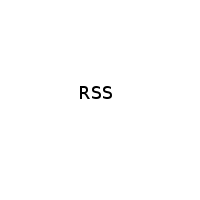
\includegraphics[width=0.5\textwidth]{figures/rss}
\caption{\label{rss-example-figure}An example of a RSS}
\end{figure}

One of possible BV is the Rectangular Swept Sphere (RSS), which is generated by sweeping a sphere (with a positive radius) over a rectangle in 3D space. The resulting volume looks something like a pillow. For an example, see figure \ref{rss-example-figure}. 

I will in this project attempt to implement a reasonably effective RSS BV, with the ability to test for overlap detection, the ability to create a new RSS from a set of points, and the ability to crate a new RSS that contains all the points of 2 (possibly disjoint) RSS'.

\subsection{Scope and Limitations}
\label{scope}
I will not try to implement the RSS in the BVH, and as a consequence not perform tests on it based on active folding of proteins, though I will test it on provided test data derived from snapshots of protein folding.

\subsection{Expectations to the reader}
I expect the reader to have a good grasp of computational geometry and, vector manipulations, and algorithms in general.

\subsection{Terminology}
In this report I will use the term ``tight fit'' to mean that the Bounding Volume around a point-set contains all the points within it, and that it has as little wasted space - i.e. regions of the BV with no points in it, as possible. BV A is a tighter fit than BV B, if both BV's contain all the points, but BV A has a smaller volume than BV B.

\subsection{Guide to this report}
\begin{description}
\item[Section \ref{introduction}] The introduction to the report, which will introduce the subject and explain my goals
\item[Section \ref{rss}] A description of the Rectangular Swept Spheres - how they are defined in theory, and how I have chosen to represent them. This section will also contain information about some of the literature that has worked with RSS.
\item[Section \ref{algorithms}] The algorithms that work on the RSSs, and an analysis of their run time 
\item[Section \ref{implementation}] Notes on the implementation of the algorithms from the previous section and the RSS itself in ProGAL.
\item[Section \ref{results}] A discussion about the results of the implementation together with a comparison with Oriented Bounding Boxes. 
\item[Section \ref{conclusion}] The conclusion of the report, where I will sum up my findings 
\end{description}



\Sfixme{Make introduction conclusion}
